\section{Pre-Supernova Abundance Analysis of Fundamental Elements}

\subsection{General Trends in \(^{12}\)C }
Across all masses, the cumulative $^{12}$C yield does not vary monotonically with metallicity. Instead, for a given CBM efficiency the yield tends to peak at an intermediate metallicity and decline at both higher and lower $Z$. In our models:
\begin{itemize}
    \item At solar metallicity ($Z = Z_\odot$), the high initial CNO content leads to rapid hydrogen burning, which limits the extent of helium burning and results in somewhat lower $^{12}$C yields.
    \item Intermediate metallicities (e.g., around $Z = 10^{-4}$ or $10^{-5}$) often optimize carbon production by striking a balance between sufficient seed nuclei and favorable core conditions.
    \item Zero-metallicity models ($Z = 0$) show intermediate yields, as carbon is produced primarily through the triple-alpha process in the absence of pre-existing heavy elements.
\end{itemize}
Notably, when comparing across masses, the 25 $M_\odot$ models generally produce higher total $^{12}$C yields than the 15 or 20 $M_\odot$ models, reflecting the more energetic core conditions in higher mass stars. However, the relative influence of metallicity and CBM remains qualitatively similar.

\subsubsection{Impact of Convective Boundary Mixing (CBM)}
Enhanced CBM increases the overall $^{12}$C yield by promoting more extensive mixing of helium into the core, which prolongs helium burning and facilitates carbon synthesis. For all three mass groups:
\begin{itemize}
    \item Models with higher CBM rates (e.g., 5\%) consistently yield higher cumulative carbon masses and exhibit smoother, more extended $^{12}$C profiles.
    \item In contrast, models with lower CBM efficiencies (e.g., 0.5\%) show yields that are more centrally concentrated, with steep gradients at the convective boundaries.
\end{itemize}
This effect is particularly significant at lower metallicities, where enhanced mixing can partially compensate for the lower initial carbon content by transporting the limited $^{12}$C outward more efficiently.

\subsubsection{Radial Distribution of $^{12}$C Mass Fraction}
The $^{12}$C mass fraction profiles provide insight into the internal distribution of carbon at core collapse:
\begin{itemize}
    \item In all models, $X_{12C}$ is highest in the helium-burning core and declines sharply at the boundary between convective and radiative regions.
    \item With stronger CBM, the $X_{12C}$ profile becomes smoother, and carbon is mixed into the outer layers, resulting in higher surface mass fractions.
    \item Although lower metallicity models naturally produce less carbon, high CBM rates can enhance the $^{12}$C mass fraction in the envelope, illustrating an important interplay between mixing and initial composition.
\end{itemize}

\subsubsection{Comparative Plots of M$_{12}C$ vs.\ $\log(Z)$}

\begin{itemize}
    \item \textbf{Non-monotonic Dependence on $Z$:} 
    Across all masses, $M_{12C}$ does not consistently increase or decrease with metallicity; instead, many models display a peak yield at an intermediate $Z$ (e.g., $10^{-4}$ or $10^{-5}$), with lower yields at both higher ($Z_\odot$) and lower ($10^{-7}$, $Z=0$) metallicities.

    \item \textbf{Impact of CBM Rate:} 
    In general, higher CBM rates produce greater carbon yields. The 5\% CBM lines (black) sit above the 2\% (red) and 0.5\% (blue) curves in most cases, reflecting how enhanced mixing extends the helium-burning core and transports newly synthesized carbon outward more efficiently.

    \item \textbf{Mass-Dependent Trends:} 
    Comparing the three panels reveals that the 25 $M_\odot$ models often achieve significantly higher $M_{12C}$ than their 15 or 20 $M_\odot$ counterparts at the same metallicity and CBM rate. This behavior highlights the more energetic core conditions in higher-mass stars, which favor stronger carbon production.

    \item \textbf{Zero-Metallicity and Very Low $Z$:}
    Even at $Z=0$, the final carbon yield can be substantial, especially when CBM rates are high (2\% or 5\%). This result underscores the role of primary nucleosynthesis (triple-alpha) in generating carbon in primordial or extremely metal-poor environments, provided that mixing is sufficiently effective.
\end{itemize}

Overall, these comparative plots emphasize the intertwined effects of metallicity, mass, and mixing efficiency on carbon synthesis. While intermediate metallicities often yield the most carbon, stronger CBM can compensate for very low $Z$, and higher-mass stars are more sensitive to changes in both composition and mixing. The net result is a highly non-linear relationship between $\log(Z)$ and $M_{12C}$, reflecting the complexity of late-stage stellar evolution in massive stars.

\subsubsection{Summary of Key Observations}
\begin{itemize}
    \item \textbf{Metallicity Dependence:} For each mass, carbon yields peak at intermediate metallicities and decline at both very high and very low $Z$. The absolute yields are higher in more massive stars.
    \item \textbf{CBM Effects:} Increased convective boundary mixing boosts both the total carbon yield and its outward transport, with the effect being most pronounced at low metallicities.
    \item \textbf{Mass Influence:} While the qualitative trends with metallicity and CBM are similar across 15, 20, and 25 $M_\odot$ models, the higher mass models (especially 25 $M_\odot$) exhibit a greater sensitivity to mixing, leading to significantly higher cumulative yields.
    \item \textbf{Combined Impact:} The final $^{12}$C distribution in pre-supernova models is determined by a complex interplay among initial mass, metallicity, and convective boundary mixing efficiency, all of which have important implications for the chemical enrichment of the interstellar medium.
\end{itemize}



%12C_M_and_CBM_Comparison
\begin{figure}
   \centering
   \begin{minipage}{0.7\textwidth}
      \centering
      \includegraphics[width=\textwidth]{12C_Mass_Fracs/15M/M12C vs Mr CBM_Comparison.png}
      \label{fig:12C_15M_VCBM}
   \end{minipage}
   \vspace{-1em}
   
   \begin{minipage}{0.7\textwidth}
      \centering
      \includegraphics[width=\textwidth]{12C_Mass_Fracs/20M/M12C vs Mr CBM_Comparison.png}
      \label{fig:12C_20M_VCBM}
   \end{minipage}
   \vspace{-1em}
   
   \begin{minipage}{0.7\textwidth}
      \centering
      \includegraphics[width=\textwidth]{12C_Mass_Fracs/25M/M12C vs Mr CBM_Comparison.png}
      \label{fig:12C_25M_VCBM}
   \end{minipage}
   \vspace{-1em}

   \caption{ \(^{12}\)C Mass Yield Comparisons for 15, 20 and 25M\(_\odot\) star respectively.}
   \label{fig:15M_yield_comparison}
\end{figure}

\clearpage
\subsection{General Trends in $^{14}$N Yields}

\subsubsection{Metallicity Dependence}  
\begin{itemize}
    \item \textbf{High $Z$ (e.g., $Z_\odot, 10^{-3}$):} 
    The presence of abundant CNO nuclei significantly enhances nitrogen production via the CNO cycle, often leading to higher $M_{14N}$. In all three mass ranges (15, 20, 25 $M_\odot$), solar and near-solar metallicities consistently yield the largest amounts of $^{14}$N.
    \item \textbf{Low/Zero $Z$ (e.g., $10^{-7}, 0$):} 
    Here, $^{14}$N synthesis relies on primary nucleosynthesis—initially forming carbon and oxygen through triple-alpha and subsequent $\alpha$-capture before nitrogen can be produced. As a result, metal-poor stars yield less $^{14}$N overall, though non-negligible amounts can still form if conditions allow.
\end{itemize}

\subsubsection{Effect of Stellar Mass:}  
\begin{itemize}
    \item \textbf{15 $M_\odot$:} 
    Nitrogen yields tend to track metallicity closely, with a moderate but noticeable boost from increased CBM. These stars produce sufficient CNO elements for an active cycle, yet their smaller cores limit the total $M_{14N}$ relative to more massive models.
    \item \textbf{20 $M_\odot$:} 
    Slightly higher core temperatures and densities lead to greater overall $^{14}$N production than in 15 $M_\odot$ stars under comparable conditions. The interplay of metallicity and CBM can create more pronounced differences in final yields.
    \item \textbf{25 $M_\odot$:} 
    The most massive models show the greatest sensitivity to mixing and metallicity, often exhibiting the widest range of $M_{14N}$ values. Strong CBM and intermediate/high $Z$ can lead to substantially elevated nitrogen yields, reflecting the vigorous nuclear burning in these stars.
\end{itemize}

\subsubsection{Influence of CBM Rates:}  
\begin{itemize}
    \item \textbf{Low CBM (0.5\%):} 
    Nitrogen-rich layers remain closer to the core, resulting in a more localized production zone. Yields are lower overall, particularly in metal-poor models.
    \item \textbf{Intermediate CBM (2\%):} 
    Enhanced mixing broadens the helium-burning region and redistributes CNO nuclei, increasing $M_{14N}$ for most metallicities. The effect is more apparent in higher-mass stars, which have larger convective cores.
    \item \textbf{High CBM (5\%):} 
    The most substantial nitrogen production occurs with 5\% CBM, especially at intermediate to high metallicities. Even low-$Z$ models see a boost in $M_{14N}$ due to the more efficient transport of newly formed carbon and oxygen, which subsequently feeds the CNO cycle.
\end{itemize}

\subsubsection{Radial Distribution of $^{14}$N Mass Fraction}

\textbf{1. Core vs. Envelope:}  
In all masses and metallicities, $X_{14N}$ peaks in or near the helium-burning core, where the CNO cycle is most active. Without strong mixing, nitrogen remains confined to this region. As CBM rates increase, nitrogen is carried into outer layers, creating smoother abundance gradients.

\textbf{2. Metallicity Influence:}  
\begin{itemize}
    \item \textbf{High $Z$:} 
    Significant $^{14}$N enrichment occurs throughout the core and into the envelope, especially with 5\% CBM, leading to relatively flat abundance profiles at larger radii.
    \item \textbf{Low $Z$:} 
    At very low or zero metallicity, the star must first synthesize carbon and oxygen before nitrogen can form. Higher CBM partially compensates by mixing these elements outward, but overall $X_{14N}$ remains modest relative to high-$Z$ stars.
\end{itemize}

\textbf{3. Mass Effects on Distribution:}  
Larger cores in 20 and 25 $M_\odot$ stars facilitate more extended burning zones, thus producing and distributing $^{14}$N over a broader radial range. In contrast, 15 $M_\odot$ models often show steeper gradients unless mixing is particularly strong (5\% CBM).

\subsubsection{Summary of Key Observations}

\begin{itemize}
    \item \textbf{Peak Yields at High/Intermediate $Z$:} 
    Regardless of mass, stars with solar or near-solar metallicities produce the most $^{14}$N, benefiting from an ample initial CNO reservoir. Intermediate metallicities can also yield robust nitrogen if the star’s core conditions and mixing rates are favorable.
    \item \textbf{Sensitivity to CBM:} 
    Stronger convective boundary mixing (2--5\%) consistently raises $M_{14N}$ across all masses and metallicities, smoothing radial abundance profiles and boosting outer-layer nitrogen content.
    \item \textbf{Mass Dependence:} 
    While the overall trends hold for 15, 20, and 25 $M_\odot$ stars, higher-mass models (especially 25 $M_\odot$) display the largest absolute yields and the greatest range of $^{14}$N production, reflecting their more energetic core environments.
    \item \textbf{Low $Z$ Production:} 
    Although $^{14}$N yields are naturally lower at $Z \approx 0$, strong mixing can partially offset the lack of seed nuclei, enabling metal-poor stars to synthesize measurable amounts of nitrogen.
\end{itemize}

%14N_M_and_CBM_Comparison
\begin{figure}
   \centering
   
   \begin{minipage}{0.7\textwidth}
      \centering
      \includegraphics[width=\textwidth]{14N_Mass_Fracs/15M/M14N vs Mr CBM_Comparison.png}
      \label{fig:14N_15M_VCBM}
   \end{minipage}
   
   \begin{minipage}{0.7\textwidth}
      \centering
      \includegraphics[width=\textwidth]{14N_Mass_Fracs/20M/M14N vs Mr CBM_Comparison.png}
      \label{fig:14N_20M_VCBM}
   \end{minipage}
   
   \begin{minipage}{0.7\textwidth}
      \centering
      \includegraphics[width=\textwidth]{14N_Mass_Fracs/25M/M14N vs Mr CBM_Comparison.png}
      \label{fig:14N_25M_VCBM}
   \end{minipage}

   \vspace{-1em}
   \caption{\(^{14}\)N Mass Yield Comparisons for 15, 20 and 25M\(_\odot\) star respectively.}
   \label{fig:20M_yield_comparison}
\end{figure}

\clearpage
\subsection{General Trends in $^{16}$O Yields}

\subsubsection{Metallicity Dependence}
\begin{itemize}
    \item \textbf{High $Z$ (e.g., $Z_\odot, 10^{-3}$):}
    Ample initial CNO elements drive robust helium burning and $\alpha$-capture, leading to elevated $M_{16O}$. Across all three masses (15, 20, 25 $M_\odot$), near-solar metallicity models tend to produce the most oxygen, thanks to efficient nuclear processing of pre-existing metals.

    \item \textbf{Intermediate $Z$ (e.g., $10^{-4}, 10^{-5}$):}
    Some models show a peak in $^{16}$O yield at intermediate metallicities, reflecting an optimal balance between core burning conditions and available seed nuclei. This trend is slightly more pronounced in higher-mass stars, which can capitalize on stronger core temperatures and densities.

    \item \textbf{Low/Zero $Z$ (e.g., $10^{-7}, 0$):}
    Here, $^{16}$O forms primarily via triple-alpha reactions followed by $\alpha$-capture on $^{12}$C. While total yields can still be substantial, they typically lag behind high-$Z$ cases unless the CBM rate is sufficiently large to expand the helium-burning region.
\end{itemize}

\subsubsection{Impact of Stellar Mass}
\begin{itemize}
    \item \textbf{15 $M_\odot$:}
    Oxygen yields reflect a moderate interplay between metallicity and CBM. The smaller convective core relative to higher-mass stars restricts the region where $\alpha$-capture can occur, although strong mixing (5\% CBM) can still boost $M_{16O}$ significantly.
    \item \textbf{20 $M_\odot$:}
    Higher core temperatures and densities lead to generally larger $^{16}$O yields compared to 15 $M_\odot$, but the same metallicity and CBM trends hold. Intermediate metallicities or near-solar $Z$ combined with robust mixing often produce the highest oxygen yields.
    \item \textbf{25 $M_\odot$:}
    These stars show the greatest sensitivity to both composition and CBM. Their larger cores and more vigorous burning can amplify differences in $Z$ and mixing efficiency, resulting in the widest range of possible oxygen yields.
\end{itemize}

\subsubsection{Effect of CBM Rates}
\begin{itemize}
    \item \textbf{Low CBM (0.5\%):}
    Oxygen production is more localized in the core, yielding steep abundance gradients. In low-metallicity stars, $M_{16O}$ remains relatively modest, as the smaller active burning zone limits primary nucleosynthesis.
    \item \textbf{Intermediate CBM (2\%):}
    Enhanced mixing broadens the helium-burning region, increasing $M_{16O}$ across all metallicities. The effect is evident for each mass, but more so in 20 and 25 $M_\odot$ models with larger cores.
    \item \textbf{High CBM (5\%):}
    Strong overshoot mixing maximizes oxygen yields by extending and prolonging helium burning. Even at $Z=0$, 5\% CBM can compensate for a lack of seed nuclei, raising $M_{16O}$ well above what would be possible under weaker mixing.
\end{itemize}

\subsubsection{Radial Distribution of $^{16}$O Mass Fraction}
\textbf{1. Core vs. Envelope:}  
In all masses and metallicities, $X_{16O}$ typically peaks near the helium-burning core. Without robust mixing, oxygen remains confined to deeper layers, resulting in sharp boundaries at the convective/radiative interface. As CBM rates increase, oxygen is transported into more external zones, smoothing the abundance gradient and enhancing surface enrichment.

\vspace{1em}
\textbf{2. Metallicity and Mixing Interaction}
\begin{itemize}
    \item \textbf{High $Z$:}
    Strong pre-existing CNO content drives efficient $\alpha$-capture, and high CBM spreads $^{16}$O outward, creating relatively uniform profiles in the outer envelope.
    \item \textbf{Low/Zero $Z$:}
    Oxygen must be built up from primary processes. While yields are lower, strong CBM (5\%) partially offsets the limited initial metals by expanding the effective burning region and redistributing newly formed $^{16}$O into the envelope.
\end{itemize}

\subsubsection{Summary of Key Observations}

\begin{itemize}
    \item \textbf{Metallicity Dependence:}
    Near-solar or intermediate $Z$ typically maximize oxygen yields, though extremely metal-poor stars can still produce notable $^{16}$O if mixing is sufficiently high.
    \item \textbf{Mass Effects:}
    Higher-mass stars (20 and 25 $M_\odot$) exhibit greater sensitivity to both metallicity and CBM, often achieving larger absolute yields and broader enrichment regions than 15 $M_\odot$ models.
    \item \textbf{Role of CBM:}
    Increasing CBM from 0.5\% to 5\% consistently boosts $M_{16O}$ and spreads oxygen into the outer layers. This effect is particularly crucial at low $Z$, where it compensates for the lack of initial seed nuclei.
    \item \textbf{Radial Profiles:}
    Minimal mixing confines $^{16}$O to the core, resulting in steep $X_{16O}$ gradients, while robust mixing yields smoother distributions and extends oxygen enrichment outward.
\end{itemize}


%16O_M_and_CBM_Comparison
\begin{figure}
   \centering
   \begin{minipage}{0.7\textwidth}
      \centering
      \includegraphics[width=\textwidth]{16O_Mass_Fracs/15M/M16O vs Mr CBM_Comparison.png}
      \label{fig:16O_15M_VCBM}
   \end{minipage}

   \vspace{-1em}
   \begin{minipage}{0.7\textwidth}
      \centering
      \includegraphics[width=\textwidth]{16O_Mass_Fracs/20M/M16O vs Mr CBM_Comparison.png}
      \label{fig:16O_20M_VCBM}
   \end{minipage}

   \vspace{-1em}
   \begin{minipage}{0.7\textwidth}
      \centering
      \includegraphics[width=\textwidth]{16O_Mass_Fracs/25M/M16O vs Mr CBM_Comparison.png}
      \label{fig:16O_25M_VCBM}
   \end{minipage}
   
   \vspace{-1em}
   \caption{  \(^{16}\)O Mass Yield Comparisons for 15, 20 and 25M\(_\odot\) star respectivelyr.}
   \label{fig:25M_yield_comparison}
\end{figure}

\clearpage
\section{Conclusion}

This study has demonstrated that the evolution and final nucleosynthetic yields of massive stars depend on a delicate interplay among stellar mass, initial metallicity, convective boundary mixing (CBM), and nuclear network selection. Higher masses produce hotter, denser cores that favor more vigorous burning, while richer metallicities provide a larger initial reservoir of CNO elements that drive efficient synthesis of $^{12}$C, $^{14}$N, and $^{16}$O. Enhanced CBM extends convective regions, increases core growth, and redistributes nuclear ashes outward, thereby boosting elemental yields even in metal-poor stars via primary nucleosynthesis.

In summary:
\begin{itemize}
    \item \textbf{Mass and Metallicity:} Higher-mass stars (e.g., 25 $M_\odot$) generally yield more elements than lower-mass stars, while intermediate to high metallicities optimize the production of $^{12}$C, $^{14}$N, and $^{16}$O.
    \item \textbf{Convective Mixing:} More efficient CBM (e.g., 5\%) expands the burning regions and smooths out the internal distribution of elements, compensating for low initial metallicity by enhancing primary nucleosynthesis.
    \item \textbf{Nuclear Networks:} The choice of nuclear reaction network affects core composition and burning conditions, with more extensive networks promoting stronger mixing and earlier ignition stages.
\end{itemize}

Overall, the final nucleosynthetic output is governed by a complex balance of these factors, which in turn influences the type of compact remnant formed and the star's role in galactic chemical enrichment. Understanding these interdependencies is essential for predicting the initial mass function (IMF) of remnants and the chemical evolution of galaxies. 